\section{تراکنش‌ها}
یکی از زیبایی‌های طراحی که انجام دادیم این است که نیازی به تراکنش در این سیستم با خواسته‌های
فعلی وجود ندارد! به عنوان مثال در زمان ثبت نام در درسی تنها
\lr{write}
در دیتابیس فقط در دیتابیس خود
\lr{enrollment service}
اتفاق می‌افتد. در قبل از آن صرفا یک سری درخواست به سرویس‌های دیگر داده می‌شود و چک می‌شود که آیا
کاربر شرایط اخذ درس را دارد یا خیر. اما نکته‌ای که وجود دارد این است که مثلا در همین سناریو انتخاب
واحد با این که نیازی به تراکنش نداریم ولی نیاز به
\lr{lock}
بر روی کاربر داریم. به عنوان مثال در صورتی که دو درس را به صورت همزمان پردازش کنیم ممکن
است که سقف واحد دانشجویی رد شود.
(مشکل \lr{race} رخ دهد.)

یا مثلا در سناریو ثبت نمره لازم نیست که نمره‌های بقیه‌ی دانشجویان را پاک کنیم اگر ثبت نمره‌ی یک نفر
به مشکل خورد. می‌توان آن فرد را صرفا برایش یک
\lr{incident}
ثبت کرد و بعدا آن فرد را به صورت جداگانه دوباره برایش نمره را ثبت کرد.

اما با این حال برای ثبت نام در درسی یک نمودار می‌کشیم.
این نمودار در شکل
\ref{transaction:good}
قابل مشاهده است.
\begin{figure}
    \centering
    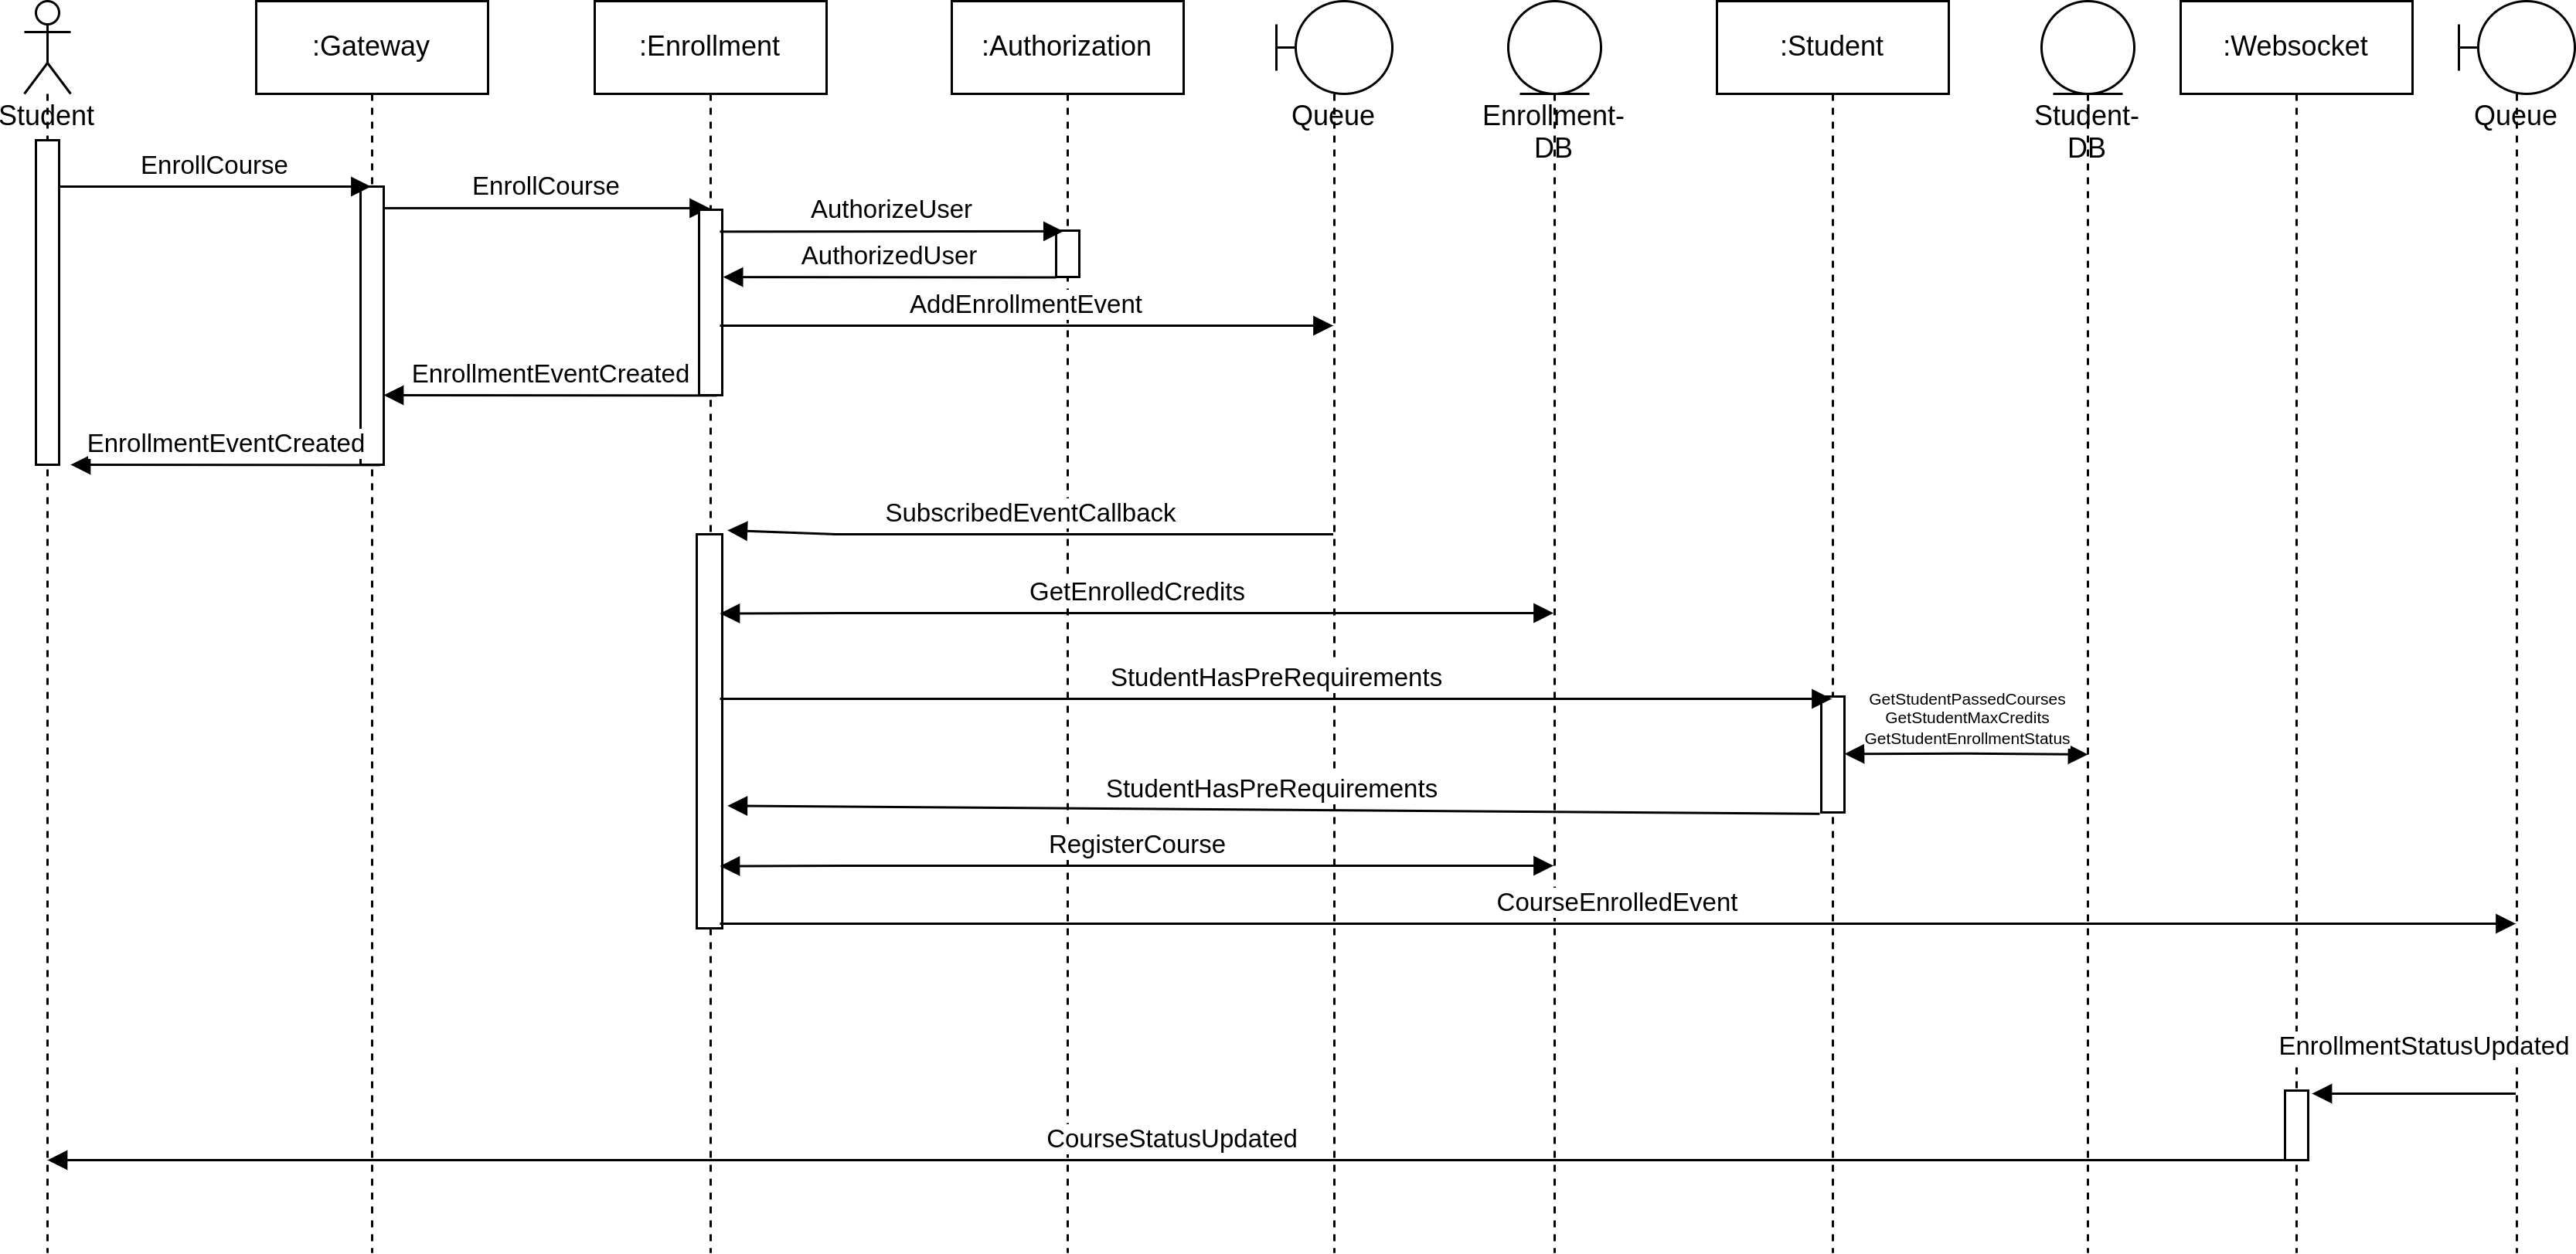
\includegraphics[width=\textwidth,height=\textheight,keepaspectratio]{diagrams/Transaction-Sucess.png}
    \caption{یک تراکنش که در آن همه چیز به خوبی پیش رفته است و چیزی \lr{fail} نشده است.}
    \label{transaction:good}
\end{figure}
همان طور که مشخص است در ابتدا درخواست از
\lr{gateway}
رد می‌شود و به سرویس
\lr{enrollment}
می‌رسد. سپس این سرویس باید توکن فرد را احراز هویت کند و در نهایت درخواست ثبت درس را در یک صف می‌فرستند.
بعدا سرویس
\lr{enrollment}
از آن صف می‌خواند و با سرویس
\lr{student}
چک می‌کند که آیا اصلا این شخص امکان برداشتن درس را دارد یا خیر. در صورتی که او مشکلی با برداشتن درس نداشت،
درس برای کاربر اخذ می‌شود که در دیتابیس خود
\lr{enrollment}
نوشته می‌شود. در نهایت یک
\lr{event}
دیگر در صف سرویس
\lr{enrollment websocket}
نوشته می‌شود. این سرویس پیام را از صف می‌خواند و برای کاربر می‌فرستند و در نتیجه کاربر می‌بیند که درس برای
اون اخذ شده است.

در ادامه یک سناریو آمده است که مثلا کاربر برای رعایت نکردن سقف واحد نمی‌تواند درس را اخذ کند
(شکل
\ref{transaction:failed}).
\begin{figure}
    \centering
    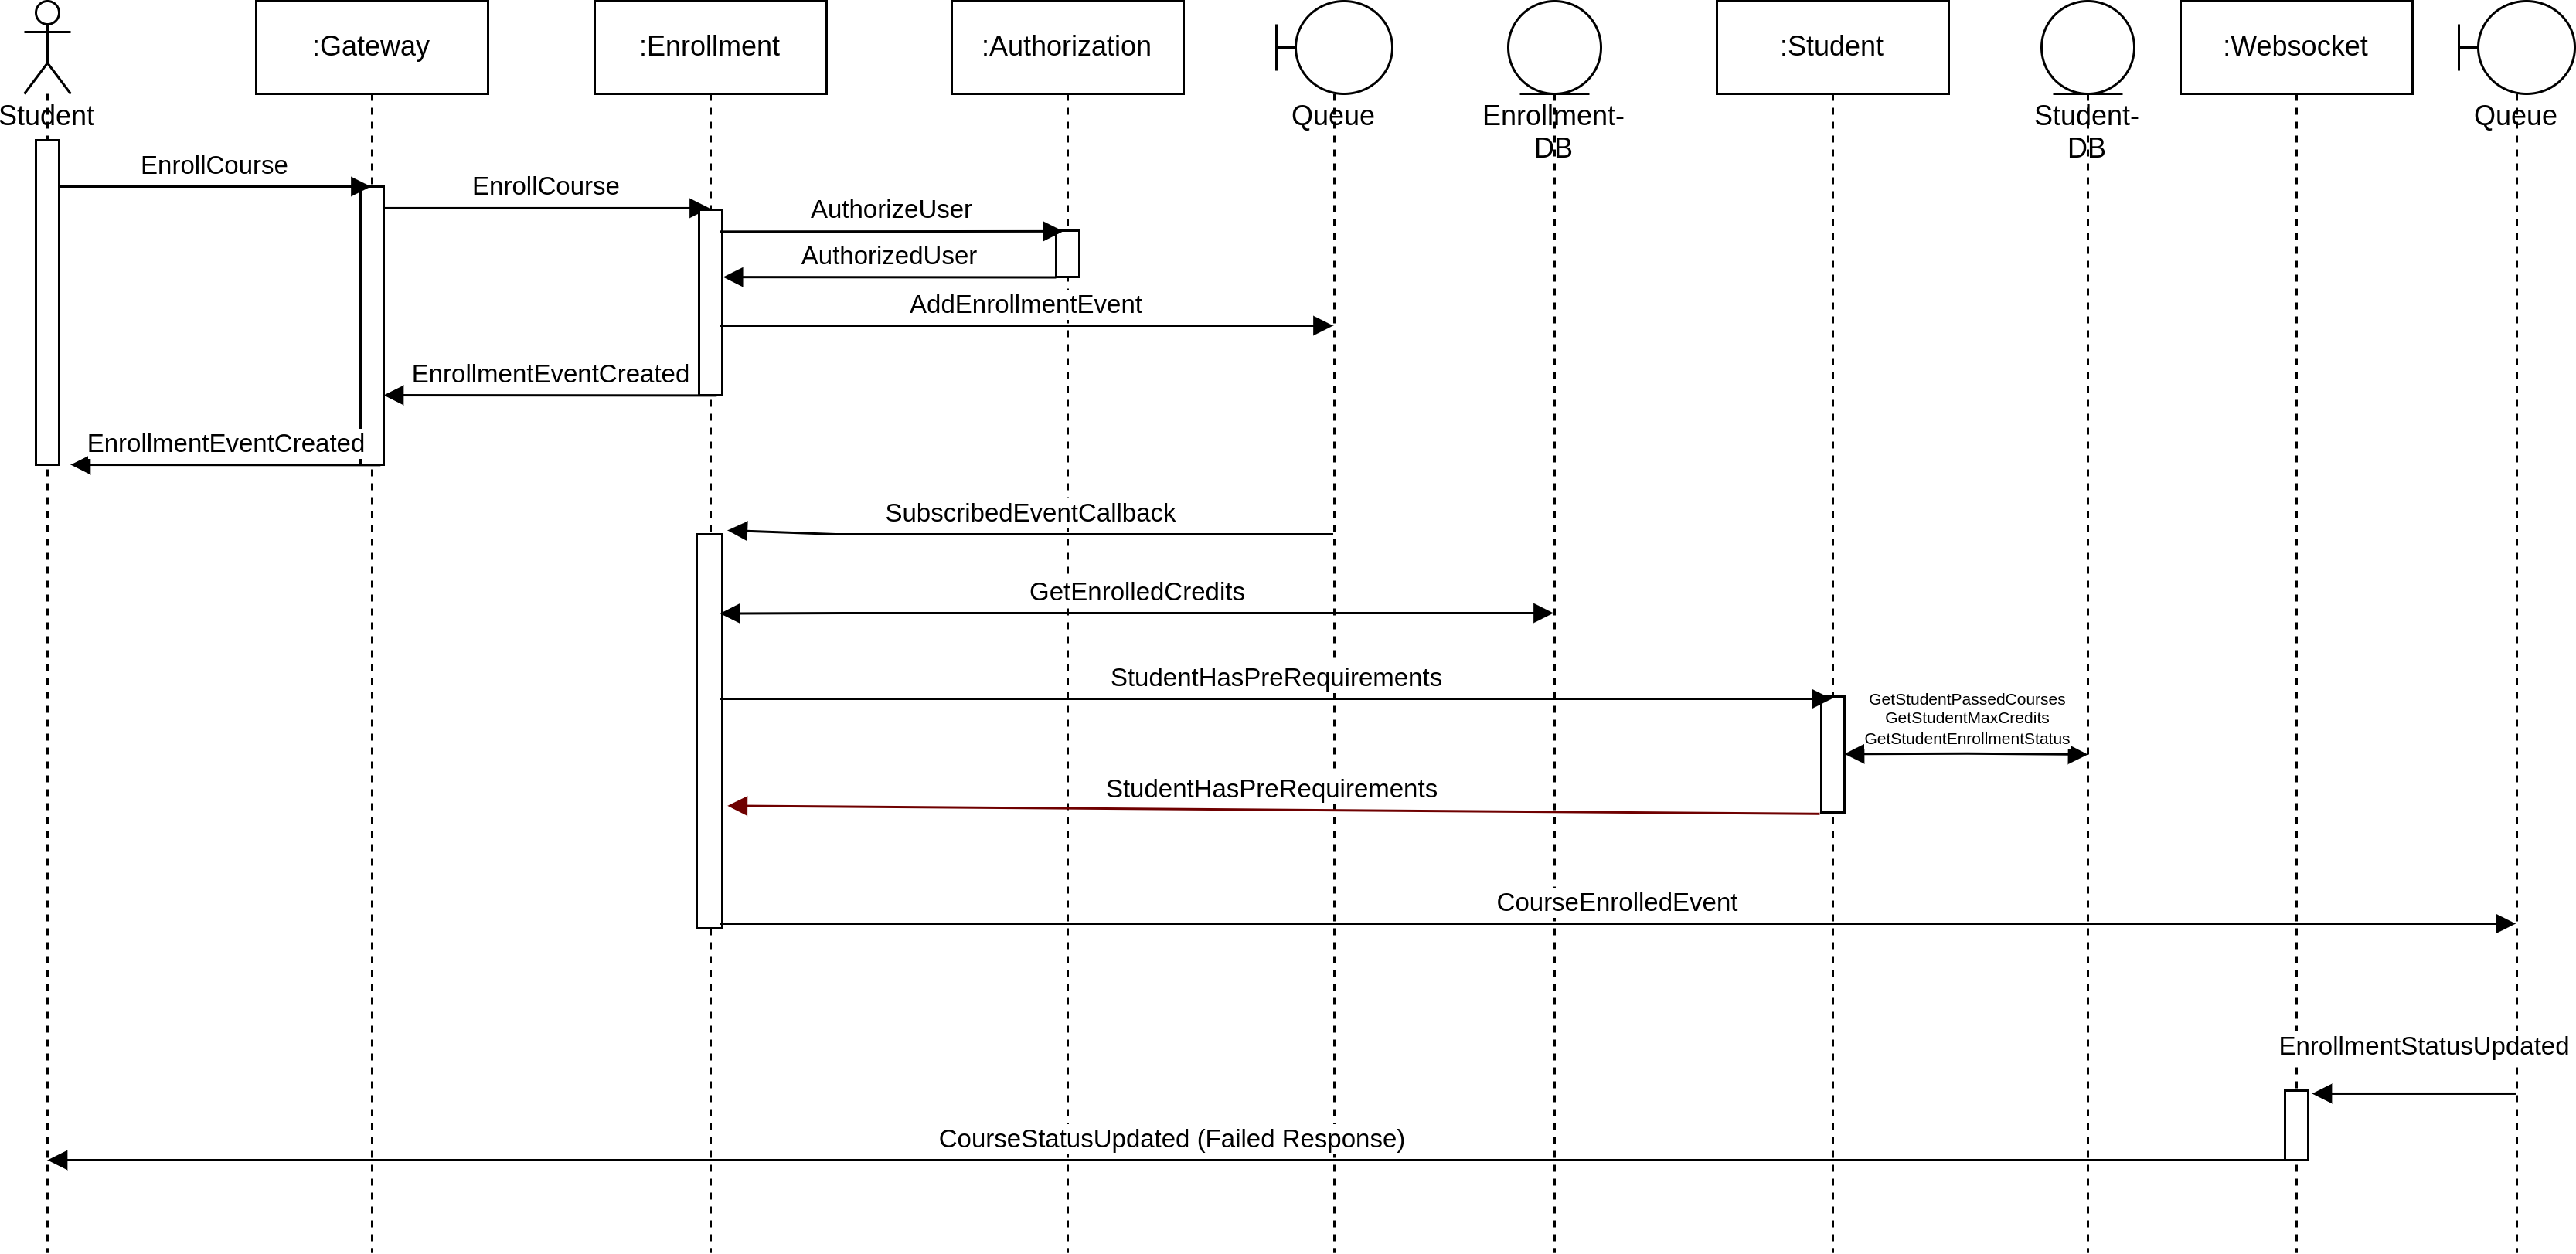
\includegraphics[width=\textwidth,height=\textheight,keepaspectratio]{diagrams/Transaction-Failed.png}
    \caption{یک تراکنش که به خاطر سقف واحد نمی‌تواند موفقیت آمیز باشد.}
    \label{transaction:failed}
\end{figure}
در این سناریو زمانی که سرویس
\lr{student}
به
\lr{enrollment}
می‌گوید که به خاطر سقف واحد درس نمی‌تواند اخذ شود، سرویس
\lr{enrollment}
چیزی در دیتابیس خود نمی‌نویسد و صرفا به سرویس
\lr{enrollment websocket}
می‌گوید که به کاربر اعلام کن که به خاطر مثلا سقف واحد نمی‌توان این درس برایش اخذ شود.